\subsection{Formelherleitung für $r$ und $Q$}
Aus der Formel \ref{eq:keinfeld} ergibt sich nach dem Einsetzen der Kraftformeln
\begin{gather*}
\frac{4}{3}\pi r^3 \rho_{Öl}\vec{g}=\frac{4}{3}\pi r^3 \rho_{L}\vec{g}+6\pi \eta  r \vec{v}_{\downarrow}\\
\iff \frac{4}{3}\pi r^3 (\rho_{Öl}-\rho_{L})\vec{g}=6\pi \eta  r \vec{v}_{\downarrow}\\
\iff r^2=\frac{9\eta \vec{v}_{\downarrow}}{2(\rho_{Öl}-\rho_{L})\vec{g}}
\iff r=\sqrt{\frac{9\eta \vec{v}_{\downarrow}}{2(\rho_{Öl}-\rho_{L})\vec{g}}}
\end{gather*}
Aus der Formel \ref{eq:mitfeld} ergibt sich nach dem Einsetzen der Kraftformeln und der Formel \ref{eq:radius}
\begin{gather*}
\frac{4}{3}\pi r^3 \rho_{Öl}\vec{g}+6\pi \eta  r \vec{v}=Q\frac{U}{d}+\frac{4}{3}\pi r^3 \rho_{L}\vec{g}\\
\iff \frac{4}{3}\pi r^3 (\rho_{Öl}-\rho_{L})\vec{g}+6\pi \eta  r \vec{v}_{\uparrow}=Q\frac{U}{d}\\
\iff Q = \frac{18 \pi d}{U}\sqrt{\frac{\eta^3 v_{\downarrow}}{2(\rho_{Öl}-\rho_L)g}}(v_{\downarrow}+v_{\uparrow})
\end{gather*}
\subsection{Zeichnung zu den Kräftegleichgewichten}
\begin{figure}[h]
  \centering
  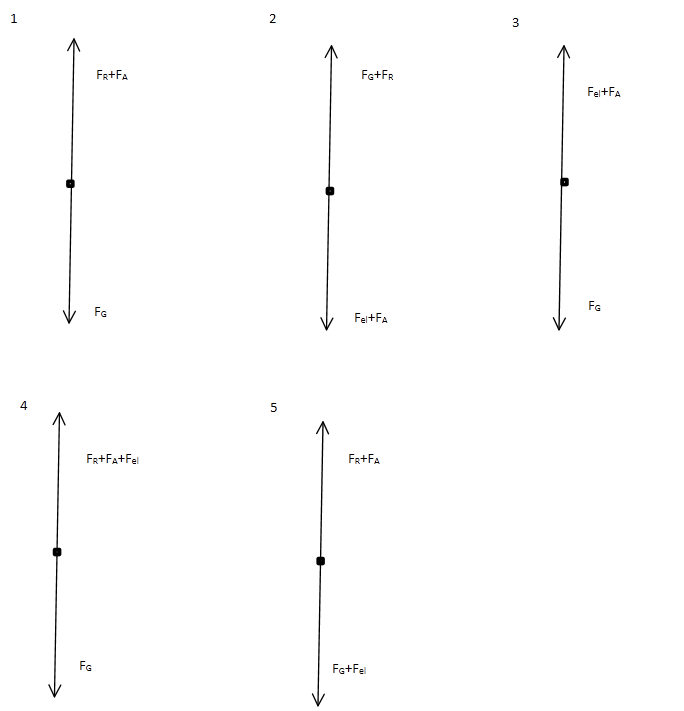
\includegraphics[width=1\textwidth]{kraftegleichgewichte.png}
  \caption{Kräftegleichgewichte}
  \label{fig:kraftegleich}
\end{figure}

\subsection{Fehlerrechnung}
Fehler für den Radius der Tröpfchen
\begin{align*}
	r &= 3 \sqrt{\frac{\eta v_\downarrow}{2(\rho_{Öl} - \rho_L)g}} \\
	\Delta r &= \left|\frac{\partial r}{\partial v_\downarrow} \Delta v_\downarrow\right| \\
	&= \frac{3}{2} \sqrt{\frac{\eta}{2(\rho_{Öl} - \rho_L)gv_\downarrow}} \Delta v_\downarrow
\end{align*}
Fehler für die Ladung des Öltröpfchens
\begin{align*}
	Q &= \frac{18\pi d}{U} \sqrt{\frac{\eta^3 v_\downarrow}{2(\rho_{Öl} - \rho_L)g}}(v_\downarrow + v_\uparrow) = \frac{6\pi\eta d}{U} r (v_\downarrow + v_\uparrow) \\
	\Delta Q &= \sqrt{\left(\frac{\partial Q}{\partial d} \Delta d\right)^2 + 
					\left(\frac{\partial Q}{\partial U} \Delta U\right)^2 + 
					\left(\frac{\partial Q}{\partial v_\downarrow} \Delta v_\downarrow\right)^2 + 
					\left(\frac{\partial Q}{\partial v_\uparrow} \Delta  v_\uparrow\right)^2} \\
	\frac{\partial Q}{\partial d} &= \frac{18\pi}{U} \sqrt{\frac{\eta^3 v_\downarrow}{2(\rho_{Öl} - \rho_L)g}}(v_\downarrow + v_\uparrow) \\
	\frac{\partial Q}{\partial U} &= -\frac{18\pi}{U^2} \sqrt{\frac{\eta^3 v_\downarrow}{2(\rho_{Öl} - \rho_L)g}}(v_\downarrow + v_\uparrow) \\
	\frac{\partial Q}{\partial v_\uparrow} &= \frac{18\pi}{U} \sqrt{\frac{\eta^3 v_\downarrow}{2(\rho_{Öl} - \rho_L)g}} \\
	\frac{\partial Q}{\partial v_\downarrow} &= \frac{18\pi}{U} \sqrt{\frac{\eta^3 v_\downarrow}{2(\rho_{Öl} - \rho_L)g}} + \frac{9\pi d}{U} \sqrt{\frac{\eta^3 }{2(\rho_{Öl} - \rho_L)gv_\downarrow}}(v_\downarrow + v_\uparrow) \\
\end{align*}